\section{Future work}

As mentioned in \cref{sec:fluorescence_microscopy}, imaging techniques -- and in particular fluorescence microscopy -- are fundamental building blocks regarding many research activities in the life sciences domain.
For this reason, we believe the field may highly benefit from the adoption of the available solutions presented in the literature concerning Deep Learning.
At the same time, the peculiar traits of the images studied in life sciences -- such as specific luminance conditions, biological and technical artifacts and cell overcrowding -- may pose stimulating challenges for deep learning researchers.
As a result, similar applications to the one described in \cref{partI} embrace potentially compelling problems for both communities. Therefore, the rest of this section is dedicated to outlining possible follow-ups we envision for the presented work.

A peculiar characteristic of microscopic fluorescence lies in the opportunistic association between the marker and the fluorophore.
Although the choice of the former depends on the experiment's goal -- since the marker must be compatible with the biological structures of interest --, the latter benefits from more freedom instead.
In particular, its choice is not bound by biological properties, meaning that different fluorophores may be associated with the same marker.
As a result, different studies may produce pictures of the same structures stained with different colors, and automatic detection approaches ought to recognize objects based on morphology rather than color.
Clearly, this poses an interesting research line aimed at investigating the invariance of different techniques to the hue information.
In this respect, a simple angle to address this requirement may be to start with grayscale images or incorporate hue-shift transformations in the augmentation pipeline.

Another interesting problem is the comparison of different strategies for precise localization. In fact, a limitation of our approach is the likely need for application-specific tuning of the post-processing parameters, especially for the watershed.
This, of course, hinders a straight transposition of the method to new use cases and paves the way for the exploration of more or less substantial variants.
A possible approach would be to experiment with alternative post-processing strategies, perhaps including their parameters in the learning process to automate their optimization (see for example \citeNP{wolf2017learned}).
Furthermore, a possible strategy to tackle this issue is to tweak the model to enforce more refined localization in the first place.
An attempt in this direction is currently under investigation by the authors of this work.
In particular, preliminary results have shown that changing from the \texttt{keras} initialization of the batch normalization layers -- \textbox{momentum=0.01, eps=0.001} -- to that adopted by \texttt{fastai} \cite{2020fastai} -- \textbox{momentum=0.1, eps=1e-5} -- seem to produce predictions with sharper boundaries (cf. top and bottom rows in \cref{fig:kerasVSfastai_bathnorm}).
\begin{figure}
\centering
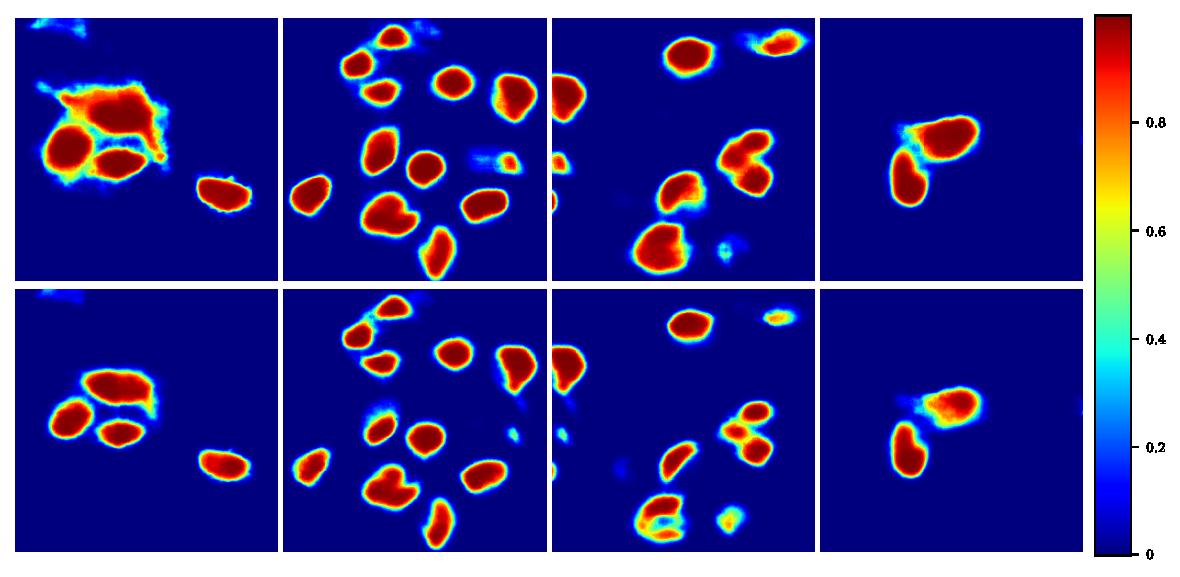
\includegraphics[width=\textwidth]{figures/610_future_works/Tc-ResUnetVSBbatchnorm_effect.pdf}
\caption{\textbf{Weight map effect}. 
Predicted heatmaps obtained with c-ResUnet using \texttt{keras} (top) and \texttt{fastai} (bottom) default initializations of the \texttt{BatchNorm} layers.} 
\label{fig:kerasVSfastai_bathnorm}
\end{figure}

Apart from variants of the study discussed in \cref{partI} of this thesis, a whole new set of experiments may be devoted to analyzing different data from those contained in the current version of the Fluorescent Neuronal Cells dataset.
In particular, we are currently studying the release of an extended dataset where more pictures are available.
These features two additional target biological structures, and the images are reported both in single exposure and with more markers visible at the same time.
This opens to novel learning tasks such as non-binary classification (one signal class per image, but more than two classes in total), multi-label classification (double marked pictures, more than one signal class in the same image) and transfer learning of the pre-trained architecture to the additional biological structures.
Also, another fascinating research direction would be to consider new data referring to different markers as a natural domain shift. Given this framework, it would be interesting to explore the extension of our approach in the context of active learning, thus aiming to enhance the model to account for additional biological structures without forgetting previous ones.
In this regard, a technical matter related to the practical implementation of the latter use case is the adoption of helpful Machine Learning Operations (MLOps) tools.
For example, this work combined \texttt{SuperAnnotate}\footnote{\superannotate} (commercial) and \texttt{Label Studio} (open source) \cite{labelstudio} to produce the visualizations presented in \cref{fig:artifacts}. Both frameworks are designed for easing MLOps pipelines and let the researchers focus on the models and the learning strategies.
The nice idea behind these tools is the concept of \textit{human in the loop}. 
Indeed, apart from easing the annotation of new data, the user can leverage such solutions to keep track of their experiments and smoothly navigate through the typical stages of practical applications, i.e. the \mbox{\textit{training $\longrightarrow$ visualization $\longrightarrow$ labels refinement $\longrightarrow$ re-training}} loop.
Also, it would be nice to integrate our codebase within powerful open source solutions for continual learning, such as the recently released \texttt{Avalanche} framework \cite{lomonaco2021avalanche}.

\begin{figure}
    \centering
    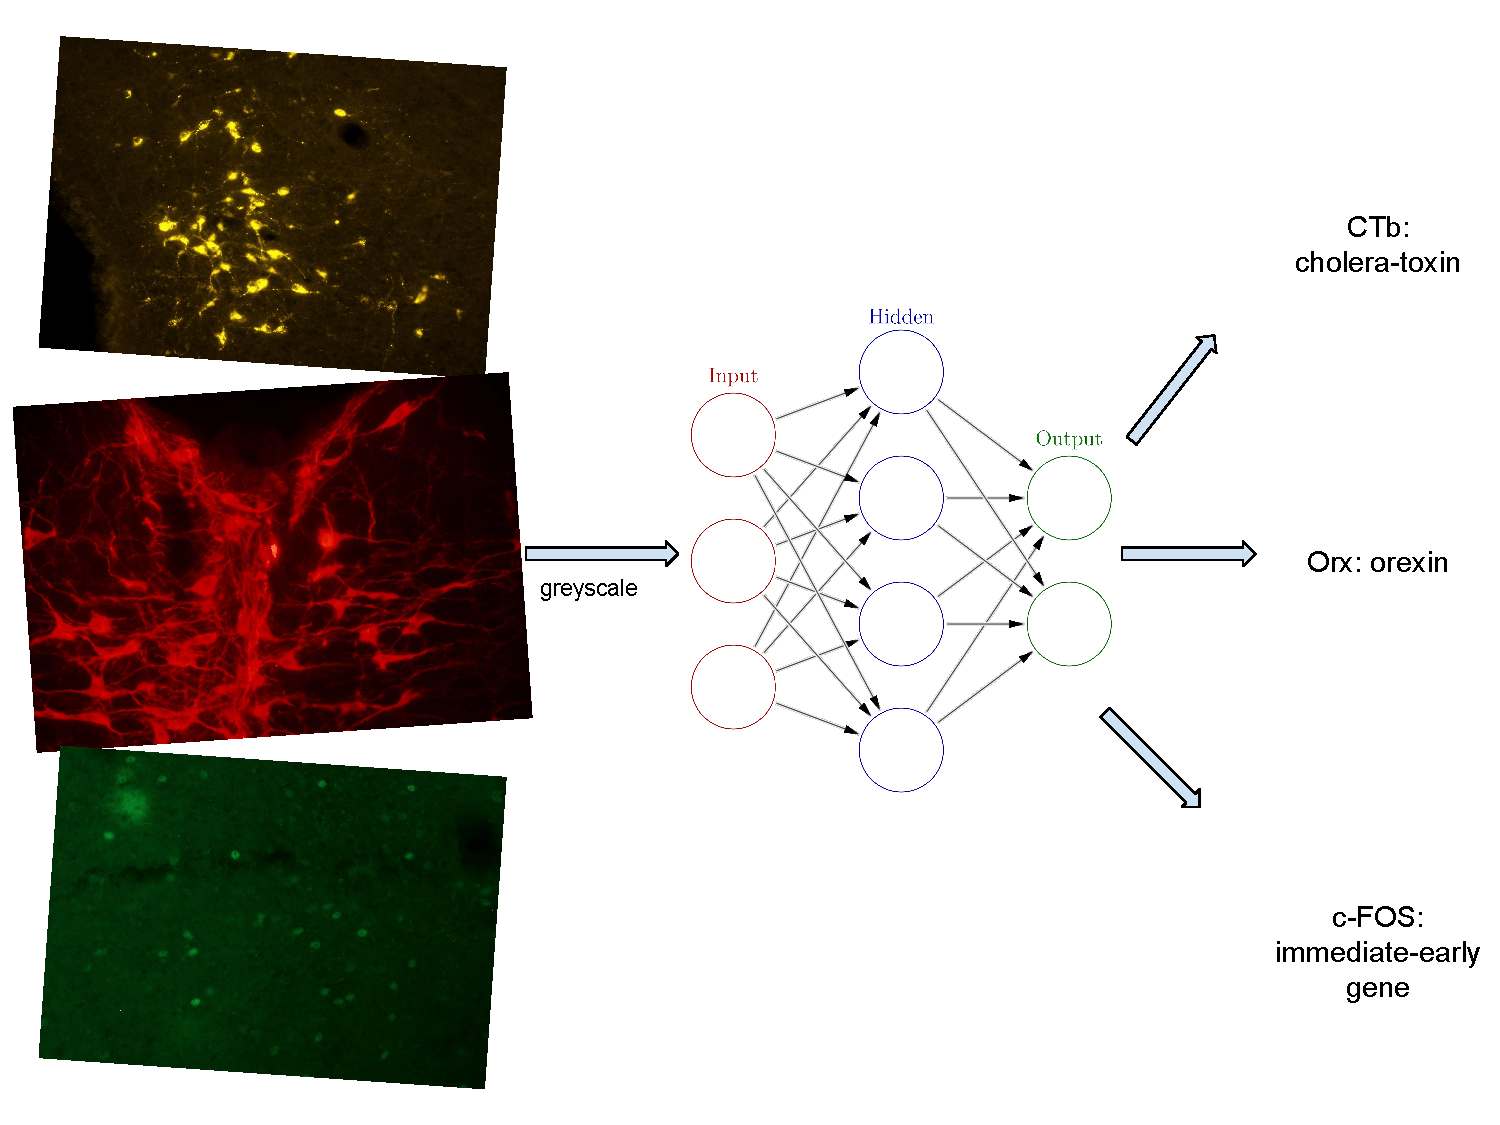
\includegraphics[width=\textwidth]{figures/610_future_works/self-supervised pretext task.pdf}
    \caption{\textbf{SSL pretext task (pre-training).} A self-supervised strategy to exploit the extended Fluorescent Neuronal Cells data. The c-ResUnet backbone is first pre-trained using marker classification as a pretext task. 
    Then, the resulting hidden representation can be leveraged for learning a downstream task of interest more easily.
    The network illustration is borrowed from  \href{https://en.wikipedia.org/wiki/Artificial_neural_network\#/media/File:Colored_neural_network.svg}{Wikipedia}
    }
    \label{fig:SSL_diagram}
\end{figure}
Despite the vast availability of fluorescence microscopy pictures, a significant bottleneck for supervised approaches is the lack of annotations. 
For this reason, a vital task would be to come up with ingenious strategies to leverage this massive amount of dispersed information without direct annotations in a \textit{Self Supervised Learning} (SSL) framework.
\Cref{fig:SSL_diagram} reports the draft of an ongoing attempt we are testing to pursue the above goal. 
In particular, we are trying to exploit the extended Fluorescent Neuronal Cells dataset to improve the encoding branch of our c-ResUnet and get rid of the weight maps. The currently studied strategy is based on a first pre-training of the c-ResUnet from scratch for marker classification. 
Specifically, the images are randomly sampled from three datasets depicting different biological structures present on the same tissues, i.e. obtained by injecting various marker-fluorophore couples into the same tissues and acquiring multiple pictures with the appropriate wavelength filtering for the corresponding marker.
Then, the single-marked images are fed grayscale into the network to predict the corresponding marker label, used as a proxy for teaching the model to discriminate images with different structures (\textit{pretext task}).
This is achieved quite easily with human-like performance.
Once that is accomplished, the same decoding path described in \cref{fig:cresunet_architecture} is attached to the end of the pre-trained encoding branch, and the model is further trained for the downstream segmentation task presented in \cref{partI}.
However, the results are not yet mature and were therefore excluded from this dissertation.

Finally, another engaging project from the data science perspective would be deploying our model in production as a service for a wider community. 
At the moment, this task is subject to a feasibility study and the collection of requirements is being conducted. These involve the development of reliable service with suitable storage and computing resources, proper access mechanism (hosting and authentication), plus efficient scalability to a reasonable number of users.